\documentclass[a4paper,12pt,twoside]{memoir}

% Castellano
\usepackage[spanish,es-tabla]{babel}
\selectlanguage{spanish}
\usepackage[utf8]{inputenc}
\usepackage[T1]{fontenc}
\usepackage{lmodern} % Scalable font
\usepackage{microtype}
\usepackage{placeins}

\RequirePackage{booktabs}
\RequirePackage[table]{xcolor}
\RequirePackage{xtab}
\RequirePackage{multirow}

% Links
\PassOptionsToPackage{hyphens}{url}\usepackage[colorlinks]{hyperref}
\hypersetup{
	allcolors = {blue}
}

% Ecuaciones
\usepackage{amsmath}

% Rutas de fichero / paquete
\newcommand{\ruta}[1]{{\sffamily #1}}

% Párrafos
\nonzeroparskip

% Huérfanas y viudas
\widowpenalty100000
\clubpenalty100000

% Imagenes
\usepackage{graphicx}
\newcommand{\imagen}[2]{
	\begin{figure}[!h]
		\centering
		\includegraphics[width=0.7\textwidth]{#1}
		\caption{#2}\label{fig:#1}
	\end{figure}
	\FloatBarrier
}

\newcommand{\imagenflotante}[2]{
	\begin{figure}%[!h]
		\centering
		\includegraphics[width=0.9\textwidth]{#1}
		\caption{#2}\label{fig:#1}
	\end{figure}
}



% El comando \figura nos permite insertar figuras comodamente, y utilizando
% siempre el mismo formato. Los parametros son:
% 1 -> Porcentaje del ancho de página que ocupará la figura (de 0 a 1)
% 2 --> Fichero de la imagen
% 3 --> Texto a pie de imagen
% 4 --> Etiqueta (label) para referencias
% 5 --> Opciones que queramos pasarle al \includegraphics
% 6 --> Opciones de posicionamiento a pasarle a \begin{figure}
\newcommand{\figuraConPosicion}[6]{%
  \setlength{\anchoFloat}{#1\textwidth}%
  \addtolength{\anchoFloat}{-4\fboxsep}%
  \setlength{\anchoFigura}{\anchoFloat}%
  \begin{figure}[#6]
    \begin{center}%
      \Ovalbox{%
        \begin{minipage}{\anchoFloat}%
          \begin{center}%
            \includegraphics[width=\anchoFigura,#5]{#2}%
            \caption{#3}%
            \label{#4}%
          \end{center}%
        \end{minipage}
      }%
    \end{center}%
  \end{figure}%
}

%
% Comando para incluir imágenes en formato apaisado (sin marco).
\newcommand{\figuraApaisadaSinMarco}[5]{%
  \begin{figure}%
    \begin{center}%
    \includegraphics[angle=90,height=#1\textheight,#5]{#2}%
    \caption{#3}%
    \label{#4}%
    \end{center}%
  \end{figure}%
}
% Para las tablas
\newcommand{\otoprule}{\midrule [\heavyrulewidth]}
%
% Nuevo comando para tablas pequeñas (menos de una página).
\newcommand{\tablaSmall}[5]{%
 \begin{table}
  \begin{center}
   \rowcolors {2}{gray!35}{}
   \begin{tabular}{#2}
    \toprule
    #4
    \otoprule
    #5
    \bottomrule
   \end{tabular}
   \caption{#1}
   \label{tabla:#3}
  \end{center}
 \end{table}
}

%
% Nuevo comando para tablas pequeñas (menos de una página).
\newcommand{\tablaSmallSinColores}[5]{%
 \begin{table}[H]
  \begin{center}
   \begin{tabular}{#2}
    \toprule
    #4
    \otoprule
    #5
    \bottomrule
   \end{tabular}
   \caption{#1}
   \label{tabla:#3}
  \end{center}
 \end{table}
}

\newcommand{\tablaApaisadaSmall}[5]{%
\begin{landscape}
  \begin{table}
   \begin{center}
    \rowcolors {2}{gray!35}{}
    \begin{tabular}{#2}
     \toprule
     #4
     \otoprule
     #5
     \bottomrule
    \end{tabular}
    \caption{#1}
    \label{tabla:#3}
   \end{center}
  \end{table}
\end{landscape}
}

%
% Nuevo comando para tablas grandes con cabecera y filas alternas coloreadas en gris.
\newcommand{\tabla}[6]{%
  \begin{center}
    \tablefirsthead{
      \toprule
      #5
      \otoprule
    }
    \tablehead{
      \multicolumn{#3}{l}{\small\sl continúa desde la página anterior}\\
      \toprule
      #5
      \otoprule
    }
    \tabletail{
      \hline
      \multicolumn{#3}{r}{\small\sl continúa en la página siguiente}\\
    }
    \tablelasttail{
      \hline
    }
    \bottomcaption{#1}
    \rowcolors {2}{gray!35}{}
    \begin{xtabular}{#2}
      #6
      \bottomrule
    \end{xtabular}
    \label{tabla:#4}
  \end{center}
}

%
% Nuevo comando para tablas grandes con cabecera.
\newcommand{\tablaSinColores}[6]{%
  \begin{center}
    \tablefirsthead{
      \toprule
      #5
      \otoprule
    }
    \tablehead{
      \multicolumn{#3}{l}{\small\sl continúa desde la página anterior}\\
      \toprule
      #5
      \otoprule
    }
    \tabletail{
      \hline
      \multicolumn{#3}{r}{\small\sl continúa en la página siguiente}\\
    }
    \tablelasttail{
      \hline
    }
    \bottomcaption{#1}
    \begin{xtabular}{#2}
      #6
      \bottomrule
    \end{xtabular}
    \label{tabla:#4}
  \end{center}
}

%
% Nuevo comando para tablas grandes sin cabecera.
\newcommand{\tablaSinCabecera}[5]{%
  \begin{center}
    \tablefirsthead{
      \toprule
    }
    \tablehead{
      \multicolumn{#3}{l}{\small\sl continúa desde la página anterior}\\
      \hline
    }
    \tabletail{
      \hline
      \multicolumn{#3}{r}{\small\sl continúa en la página siguiente}\\
    }
    \tablelasttail{
      \hline
    }
    \bottomcaption{#1}
  \begin{xtabular}{#2}
    #5
   \bottomrule
  \end{xtabular}
  \label{tabla:#4}
  \end{center}
}



\definecolor{cgoLight}{HTML}{EEEEEE}
\definecolor{cgoExtralight}{HTML}{FFFFFF}

%
% Nuevo comando para tablas grandes sin cabecera.
\newcommand{\tablaSinCabeceraConBandas}[5]{%
  \begin{center}
    \tablefirsthead{
      \toprule
    }
    \tablehead{
      \multicolumn{#3}{l}{\small\sl continúa desde la página anterior}\\
      \hline
    }
    \tabletail{
      \hline
      \multicolumn{#3}{r}{\small\sl continúa en la página siguiente}\\
    }
    \tablelasttail{
      \hline
    }
    \bottomcaption{#1}
    \rowcolors[]{1}{cgoExtralight}{cgoLight}

  \begin{xtabular}{#2}
    #5
   \bottomrule
  \end{xtabular}
  \label{tabla:#4}
  \end{center}
}



\graphicspath{ {./img/} }

% Capítulos
\chapterstyle{bianchi}
\newcommand{\capitulo}[2]{
	\setcounter{chapter}{#1}
	\setcounter{section}{0}
	\setcounter{figure}{0}
	\setcounter{table}{0}
	\chapter*{#2}
	\addcontentsline{toc}{chapter}{#2}
	\markboth{#2}{#2}
}

% Apéndices
\renewcommand{\appendixname}{Apéndice}
\renewcommand*\cftappendixname{\appendixname}

\newcommand{\apendice}[1]{
	%\renewcommand{\thechapter}{A}
	\chapter{#1}
}

\renewcommand*\cftappendixname{\appendixname\ }

% Formato de portada
\makeatletter
\usepackage{xcolor}
\newcommand{\tutor}[1]{\def\@tutor{#1}}
\newcommand{\course}[1]{\def\@course{#1}}
\definecolor{cpardoBox}{HTML}{E6E6FF}
\def\maketitle{
  \null
  \thispagestyle{empty}
  % Cabecera ----------------
\noindent
\includegraphics[width=\textwidth]{cabecera}\vspace{1cm}%
  \vfill
  % Título proyecto y escudo informática ----------------
  \colorbox{cpardoBox}{%
    \begin{minipage}{.8\textwidth}
      \vspace{.5cm}\Large
      \begin{center}
      \textbf{TFG del Grado en Ingeniería Informática}\vspace{.6cm}\\
      \textbf{\LARGE\@title{}}
      \end{center}
      \vspace{.2cm}
    \end{minipage}

  }%
  \hfill\begin{minipage}{.20\textwidth}
    
\includegraphics[width=\textwidth]{escudoInfor}
  \end{minipage}
  \vfill
  % Datos de alumno, curso y tutores ------------------
  \begin{center}%
  {%
    \noindent\LARGE
    Presentado por \@author{}\\ 
    en Universidad de Burgos --- \@date{}\\
    Tutor Académico: \@tutor{}\\
    Tutor Empresarial (ITCL): Alejandro Langarica Aparicio\\
  }%
  \end{center}%
  \null
  \cleardoublepage
  }
\makeatother

\newcommand{\nombre}{Víctor de la Iglesia García} %%% cambio de comando

% Datos de portada
\title{Control Robótico mediante Tecnologías Inmersivas }
\author{\nombre}
\tutor{Carlos Cambra Baseca}

\date{\today}

\begin{document}

\maketitle


\newpage\null\thispagestyle{empty}\newpage


%%%%%%%%%%%%%%%%%%%%%%%%%%%%%%%%%%%%%%%%%%%%%%%%%%%%%%%%%%%%%%%%%%%%%%%%%%%%%%%%%%%%%%%%
\thispagestyle{empty}


\noindent
\includegraphics[width=\textwidth]{cabecera}\vspace{1cm}

\noindent D. Carlos Cambra Baseca, profesor del departamento de Ingeniería Informática, área de Ciencia de la Computación e Inteligencia Artificial.

\noindent Expone:

\noindent Que el alumno D. \nombre, con DNI 71365599A, ha realizado el Trabajo final de Grado en Ingeniería Informática titulado Control Robótico mediante Tecnologías Inmersivas. 

\noindent Y que dicho trabajo ha sido realizado por el alumno bajo la dirección del que suscribe, en virtud de lo cual se autoriza su presentación y defensa.

\begin{center} %\large
En Burgos, {\large \today}
\end{center}

\vfill\vfill\vfill

% Author and supervisor
\begin{minipage}{0.45\textwidth}
\begin{flushleft} %\large
Vº. Bº. del Tutor:\\[2cm]
D. Carlos Cambra Baseca
\end{flushleft}
\end{minipage}
\hfill
\begin{minipage}{0.45\textwidth}
\begin{flushleft} %\large
Vº. Bº. del tutor:\\[2cm]
D. Alejandro Langarica Aparicio
\end{flushleft}
\end{minipage}
\hfill

\vfill

% para casos con solo un tutor comentar lo anterior
% y descomentar lo siguiente
%Vº. Bº. del Tutor:\\[2cm]
%D. nombre tutor


\newpage\null\thispagestyle{empty}\newpage




\frontmatter

% Abstract en castellano
\renewcommand*\abstractname{Resumen}
\begin{abstract}
A lo largo de todo este documento es recogida la información fundamental relativa al desarrollo de un software que permita al usuario el teleoperar un brazo robótico, con alguna funcionalidad más. 

Utilizando un dispositivo de realidad virtual como son las gafas Oculus Quest 2, unos guantes hápticos SenseGlove Nova y un ordenador con el motor gráfico Unity podremos desplazar gracias a este software la pinza de un brazo robótico a lo largo de las tres dimensiones del espacio, permitiendo además abrir o cerrar esta pinza mediante gestos con una de nuestras manos.

Este proyecto ha sido desarrollado desde Unity haciendo uso del lenguaje C\# para la creación de scripts, y de otras herramientas y plugins. Todo este material usado, además de las instalaciones para llevarlo a cabo son del Instituto Tecnológico de Castilla y León.

Este proyecto sirve y servirá como base para el desarrollo por parte de la empresa de uno de dimensiones mucho más grandes para el que queda todavía mucho tiempo de evolución.
\end{abstract}

\renewcommand*\abstractname{Descriptores}
\begin{abstract}
Unity, Oculus Quest 2, realidad virtual, tecnología háptica, robótica, C\# 
\end{abstract}

\clearpage

% Abstract en inglés
\renewcommand*\abstractname{Abstract}
\begin{abstract}
Throughout this document, the fundamental information related to the development of a software that allows the user to teleoperate a robotic arm, with some more functionalities, is collected.

Thanks to this software and using a virtual reality device such as the Oculus Quest 2 glasses, SenseGlove Nova haptic gloves and a computer with the Unity graphics engine, you can move the gripper of a robotic arm along the three dimensions of space, allowing also to open or close this clip by gestures with one of our hands.

This project has been developed from Unity using the C\# language to create scripts, and other tools and plugins. All this material used, in addition to the facilities to carry it out, are from the Technological Institute of Castilla y León.

This project serves and will serve as the basis for the development by the company of one of much larger dimensions for which there is still a long time to evolve.

\end{abstract}

\renewcommand*\abstractname{Keywords}
\begin{abstract}
Unity, Oculus Quest 2, Virtual Reality, haptic technology, robotics, C\#
\end{abstract}

\clearpage

% Indices
\tableofcontents

\clearpage

\listoffigures

\clearpage


\mainmatter
\capitulo{1}{Introducción}
En pleno siglo XXI, hemos podido ir observando como casi día a día las nuevas soluciones tecnológicas desarrolladas van cubriendo más y más necesidades de nuestra sociedad. Estas soluciones también avanzan en cuanto a la manera de ser controladas y gestionadas. Hasta la fecha la gran mayoría de los robots que son utilizados de manera teleoperada han sido controlados a través de joysticks, paneles de mandos o teclados. En cuanto a la visión, la manera de gestionarla convencionalmente ha sido desde monitores o pantallas. 

A día de hoy, la tecnología nos da la posibilidad de vivir esta experiencia de control a distancia de una forma mucho más inmersiva y es ahí donde está el motivo que da alas a este proyecto. Se realizó un estudio del interés posible por las empresas en este tipo de tecnologías y este fue muy amplio. El motivo de este interés proviene del hecho de que hay tareas que un robot con inteligencia artificial no es capaz de hacer de forma autónoma por la complejidad que requiere y por otro lado, son peligrosas de realizar por el ser humano. Ejemplos son tareas como la de colocar cargas explosivas en una mina, desactivar bombas, inspeccionar o tomar muestras en ambientes tóxicos, reparaciones en entornos subacuáticos o incluso, el mantenimiento de satélites en órbita. En todas estas tareas se usan robots teleoperados y cuanto mayor sea la inmersividad para el operario, mejor será desempeñada la tarea.

La idea propuesta por este TFG y desarrollado en conjunto con el Instituto Tecnológico de Castilla y León (ITCL) \cite{ITCL} nace de una idea genuina de mi tutor en la empresa, Alejandro Langarica. Y busca con él, explorar las posibilidades que nos da la tecnología para el control robótico haciendo uso de tecnología inmersiva, con dispositivos de realidad virtual\cite{VR} como Oculus Quest 2 \cite{Quest2} y los guantes hápticos Nova que usaremos en el proyecto.

\section{Estructura de la memoria}
A la hora de realizar la memoria del proyecto, este se ha dividido en los siguientes apartados para una mejor y más fácil comprensión de todo lo expuesto:
\begin{itemize}
\item \textbf{Introducción} : Ligera descripción del proyecto junto a la estructura tanto de la memoria como de los anexos.
\item \textbf{Objetivos del proyecto}: Explicación breve de los objetivos perseguidos en el desarrollo del proyecto, distinguiéndolos en principales, secundarios, técnicos y personales. 
\item \textbf{Conceptos teóricos}: Explicaciones necesarias para comprender aquellos conceptos dispuestos y utilizados en la memoria.
\item \textbf{Técnicas y herramientas}: Presentación de las técnicas, metodologías y herramientas empleadas para realizar el proyecto.
\item \textbf{Aspectos relevantes del desarrollo}: Presentación de aquellas partes más importantes y destacadas a la hora de llevar a cabo el desarrollo del proyecto.
\item \textbf{Trabajos relacionados}: Apartado donde se explican aquellos proyectos realizados y similares al expuesto en esta memoria.
\item \textbf{Conclusiones y lineas de trabajo futuras}: Explicación de aquellas conclusiones derivadas del desarrollo del proyecto, junto con la descripción de posibilidades de mejora y expansión del mismo en el futuro.
\end{itemize}


\section{Anexos}
\begin{itemize}
    \item \textbf{Plan de proyecto software} : Planificación temporal junto con los estudios de viabilidad.
    \item \textbf{Especificación de requisitos}:  Catálogo y especificación de los requisitos necesarios para desarrollar el proyecto. 
    \item \textbf{Diseño}: Aquello relacionado con el diseño del software.
    \item \textbf{Manual del programador}: Guía para la utilización de los ficheros para trabajar con ellos o continuar desarrollando.
    \item \textbf{Manual del usuario}: Guía para el uso del software a nivel de usuario.
\end{itemize}
\subsection{Materiales Añadidos}
La entrega del material correspondiente a este trabajo final de grado está compuesta por la memoria, los anexos, la carpeta contenedora del proyecto, fuentes de la documentación a través de un directorio con el proyecto de \LaTeX y un vídeo que recoge una muestra de algunos de los resultados.
\capitulo{2}{Objetivos del proyecto}

El objetivo principal buscado en este proyecto es el de realizar una aplicación software que permita al usuario el establecer comunicación entre él mismo y un dispositivo robótico, por medio de internet y usando como nexo entre ambos la realidad virtual y todo lo que nos ofrece.

En conjunto con ITCL\cite{itcl} pusimos sobre la mesa una serie de objetivos que podemos considerar como principales, ya que son aquellos que debíamos cumplir para sacar adelante el proyecto, y otros más ambiciosos con mayor dificultad y requerimiento a nivel de tiempo que podemos considerar secundarios. Por otro lado marcamos unos también a nivel técnico y yo por mi parte, unos objetivos personales a cumplir con el proyecto.

\section{Objetivos Principales}
\begin{enumerate}
    \item Comprender y ver el funcionamiento de la plataforma de desarrollo Unity\cite{Unity}.
    \item Comprender las posibilidades que nos ofrecen las gafas de realidad virtual Oculus Quest 2\cite{Quest2}.
    \item Entender el funcionamiento de los guantes hápticos SenseGlove Nova.
    \item Establecer la conexión entre los guantes y las gafas, con nuestro ordenador, para la recolección de datos con Unity.
    \item Desarrollo de software especializado con Unity que de sentido a esos datos recogidos.
    \item Conexión de Unity y nuestro ordenador con el robot Kinova a través de la red pública.
    \item Desarrollo de software para teleoperar todas las partes móviles del robot mediante nuestra tecnología de realidad virtual. 
\end{enumerate}

\section{Objetivos Secundarios}
\begin{enumerate}
    \item Conseguir, además del desplazamiento en el espacio de la pinza robot, implementar la funcionalidad de apertura y cierre de la pinza con gestos desde los guantes.
    \item Recibir respuesta háptica\cite{Haptica1} al operador en relación a variaciones en el estado del robot o su entorno.
    \item Visualizar de forma estereoscópica lo que está viendo el robot.
    \item Comandar la cámara estereoscópica del robot únicamente con los movimientos de cabeza del operador.
\end{enumerate}

\section{Objetivos Técnicos}
\begin{enumerate}
    \item Establecer la conexión inalámbrica entre todos los dispositivos involucrados en el proyecto.
    \item Aprender y entender como comunicarse con el robot.
    \item Uso de repositorios y herramientas tanto de control de versiones como de planificación/administración del proyecto.
    \item Establecer un material bien documentado, que pueda ser de utilidad a las personas interesadas en esta clase de proyectos.
\end{enumerate}

\newpage

\section{Objetivos Personales}
\begin{enumerate}
    \item Aprender a desarrollar con Unity\cite{Unity} aplicaciones para Oculus Quest 2.
    \item Aprender a desarrollar y entender el mundo de la realidad virtual\cite{VR}.
    \item Desarrollar software de manera depurada y limpia.
    \item Aprovechar los conocimientos recibidos durante la carrera en diferentes ámbitos, para fusionarlos en este proyecto.
    \item Uso de la metodología agil de desarrollo software SCRUM\cite{SCRUM}
    \item Desarrollar la documentación del proyecto mediante \LaTeX.
\end{enumerate}
\capitulo{3}{Conceptos teóricos}

A lo largo de este apartado serán expuestos aquellos conceptos a nivel teórico, necesarios de comprender tanto para el desarrollo normal del proyecto con Unity y el conjunto de dispositivos utilizados, como para entender el funcionamiento y propósito del proyecto.

Sin estas explicaciones, el desarrollo de las tareas es difícil de comprender para aquellas personas que no han trabajado previamente con estas tecnologías. 

\section{Oculus Quest 2}

En este punto de conceptos teóricos desarrollaremos todo aquello relacionado con las gafas de realidad virtual Oculus Quest 2. 

\subsection{VR: Virtual Reality}
La realidad virtual\cite{VR} se define como un entorno con escenas y objetos que simulan la realidad. Es generada mediante tecnologías informáticas que generan en el usuario una experiencia de inmersión.

Este entorno es percibido por el usuario a través de gafas o cascos de realidad virtual, que además unido a otros dispositivos como guantes o trajes, dan al usuario una mayor experiencia de interacción con el entorno y sus objetos. Dando lugar a mayor sensación de realismo.

\subsection{Oculus Quest 2}
También conocidas como Meta Quest 2 desde Noviembre de 2021. 
Son unas gafas de realidad virtual, las cuales nos permiten tanto vivir experiencias inmersivas, como desarrollarlas para otros usuarios.

Estas gafas contienen internamente, un sistema operativo basado en Android para hacer uso únicamente de ellas y además, la posibilidad de ser conectadas al software VR de Oculus que se ejecuta en un ordenador mediante Wi-Fi o USB.

Junto con las gafas, se dispone de dos controladores Touch. Uno desarrollado para cada mano y que sirven como mandos para controlar nuestras sesiones de uso de Quest 2.
Poseen un procesador Qualcomm Snapdragon™ XR2 con 6 GB de RAM, pantalla LCD de cambio rápido con alta resolución y tasa de refresco.
\imagen{Oculus-Quest-2.png}{Oculus Quest 2 con sus controladores Touch}

\subsection{Seguimiento}
Esta característica permite a los dispositivos el conocer instantáneamente la posición de manos, objetos e incluso en algunos casos, de ojos. Todo esto, mediante software y en conjunto con cámaras o sensores.

Este seguimiento se lleva a cabo mediante 4 cámaras infrarrojas colocadas en las gafas, las cuales permiten usar la tecnología de seis grados de libertad\cite{6Grados}. Seis grados de libertad hace referencia al desplazamiento dentro de un espacio de tres dimensiones, es decir, la posibilidad de movimiento hacia arriba/abajo, delante/atrás, izquierda/derecha junto con la rotación alrededor de los tres ejes perpendiculares.

Es gracias a esta tecnología que se pueda realizar un seguimiento de los movimientos de nuestra cabeza e incluso también de nuestro cuerpo, y que se pueda integrar toda esta información en la VR con una precisión totalmente realista sin necesidad de utilizar sensores externos como utilizan otros dispositivos.

\newpage

\section{SenseGlove Nova}
En este punto de conceptos teóricos desarrollaremos todo aquello relacionado con los guantes hápticos de realidad virtual SenseGlove Nova.

\subsection{Tecnología Háptica}
Háptica se refiere a “Estudio de las percepciones a través del tacto” (Real Academia Española, 23/05/2022, definición 2). Este término que lo relaciona con la tecnología hace referencia a cualquier tecnología que pueda ofrecer una experiencia de tacto con la aplicación a través de fuerzas, vibraciones o movimientos al usuario.

Con todo esto se pueden desarrollar objetos virtuales que ofrezcan sensaciones realistas al usuario, se pueden manipular de manera remota teleoperadores y asi permitir el control remoto de máquinas y dispositivos. 

\subsection{SenseGlove Nova}
 Estos guantes hápticos modelo Nova \cite{SGloveNova}, tienen como predecesores a los primeros llevados a cabo por la empresa, que nacen del trabajo final de la carrera de sus dos fundadores Johannes Luijten y Gijs den Butter, en la Universidad Tecnológica de Delft, Países Bajos.
 
 Funcionan de manera inalámbrica gracias a su batería y se pueden conectar por Bluetooth. Estos guantes están dotados de una tecnología por encima de lo frecuente hoy en día, y es ese el motivo de su alto precio de venta al público.
 
 Esta tecnología cuenta con un sensor de orientación absoluta con nueve ejes para capturar el movimiento en la muñeca. También con cuatro sensores para captar la flexión y extensión del pulgar y los dedos índice, medio y anular. Además cuenta con un sensor para capturar la abducción y aducción del pugar. 
 
 \newpage
 Para la parte de respuesta al usuario, los guantes cuentan con 4 módulos, desarrollados por ellos mismos, de retroalimentación de fuerza pasiva que ofrecen una fuerza máxima de 20N en dirección de flexión en el final de los dedos. En el lado háptico encontramos con que poseen 3 motores hápticos que funcionan emitiendo vibraciones produciendo sensaciones en el pulgar, índice y en la palma.
 
\imagen{cropped-SenseGlove-Nova-glow.png}{Guante Háptico Nova}

\newpage

\section{Kinova Robotics}
En este punto de conceptos teóricos desarrollaremos todo aquello relacionado con la tecnología robótica que utilizamos, Kinova Robotics.

\subsection{Robótica}
Este término hace referencia a la "Técnica que aplica la informática al diseño y empleo de aparatos que, en sustitución de personas, realizan operaciones o trabajos, por lo general en instalaciones industriales" (Real Academia Española, 23/05/2022, definición 2). De esta manera, podemos ver que la robótica \cite{Robotica} viene de cruzar en un mismo punto ciencia, ingeniería y tecnología. Todo esto con el fin de cada día cubrir más necesidades humanas. 

Dependiendo del tipo de tarea a cubrir, la dificultad o incluso el lugar donde ejecutar la tarea, existen robots más básicos que únicamente se encargan de tareas sencillas como desplazar objetos hasta otros que poseen tecnologías más desarrolladas con algoritmos de aprendizaje o inteligencia artificial. Estos en función de su naturaleza pueden ser automáticos o que necesiten de teleoperación y en función de sus formas les hay estáticos, móviles, o incluso antropomorfos.    

\subsection{Telerrobótica}
Dentro de la robótica existe un área dedicada a la manipulación de robots en la distancia, utilizando para la conexión muchas veces tecnologías de tipo wireless o mediante Internet.
La telerrobótica\cite{Telerrobotica} nace combinando dos terminologías:
\begin{enumerate}
    \item \textit{Teleoperación:} Hace referencia a la realización de una actividad o trabajo a distancia, que puede ser física estando a una larga distancia por ejemplo, o puede referirse a un cambio de escala, para trabajos muy precisos.
    \item \textit{Telepresencia}\cite{Telepresencia}: Referida a aquella tecnología que nos permite "transportarnos" de un espacio puramente físico a otro, a través de la red, dotándonos de la posibilidad de experimentar el estar en ese nuevo espacio, de manera virtual. 
\end{enumerate}

\subsection{Robot Kinova}
Para nuestro proyecto, hemos decidido utilizar el brazo robótico Kinova de segunda generación del que disponemos en ITCL. Este en concreto, posee una pinza de dos dedos al final del brazo, pero los hay con tres. Debido a la movilidad que posee y a sus ejes, este robot es un modelo 6DOF(Six Degrees of Freedom) lo que nos permite mover la pinza como ya hemos explicado anteriormente, siguiendo los seis grados de libertad.

En cuanto a las características técnicas de este robot, encontramos que al ser la versión con dos dedos se nos permite sostener una carga de hasta 1,8Kg. Que tiene una velocidad lineal máxima de desplazamiento de 20 cm/s, que permite conexión por puertos como USB o Ethernet. A nivel de software el desarrollo se puede hacer con Windows, Linux o ROS. En este caso, nosotros utilizamos ROS.
\imagen{kinova.jpg}{Imagen del brazo robótico Kinova} 

\subsection{ROS}
Las siglas ROS\cite{ROS} definen Robot Operating System, lo que nos indica que es un meta sistema operativo(en este caso de código abierto) para robots. Da servicios como los que serían esperados de un sistema operativo como puede ser el controlar dispositivos de bajo nivel, la abstracción de hardware, implementación de funcionalidades o el paso de mensajes entre procesos.

ROS destaca por ser ligero y así permitir su uso con otros frameworks o estructuras de desarrollo software de robots, por ser de fácil implementación en los lenguajes actuales de programación y por su fácil escalado a procesos mayores.

ROS dota de una manera de enlazar una red de procesos(llamados nodos en ROS). Estos nodos se pueden ejecutar en múltiples dispositivos y se conectan a un eje central. Los nodos se comunican entre ellos pasándose mensajes. Un nodo envía un mensaje a través de publicarlo en un topic dado. Un topic, es un nombre que se usa para identificar el contenido de un mensaje. Un nodo que esté interesado en un tipo específico de dato se suscribirá al topic apropiado. Puede haber múltiples publicadores y suscriptores para un solo topic, y un nodo puede publicar y/o suscribir a multiples topics.\imagen{ROS_basic_concepts.png}{Diagrama con conceptos básicos de ROS}

\newpage

\section{Unity}
En este punto de conceptos teóricos desarrollaremos todo aquello relacionado con el motor gráfico Unity, que ha sido utilizado para el desarrollo del proyecto.

\subsection{Motor Gráfico}
Por motor gráfico\cite{MotorGrafico} entendemos un conjunto de rutinas de programación, que nos da la posibilidad de diseñar, crear o producir los funcionamientos de un juego. Alguna de las cosas que se nos permite hacer son:
\begin{itemize}
    \item Renderizado de gráficos que vemos en pantalla.
    \item Elaboración de físicas que permiten ver como se generan las colisiones entre objetos.
    \item Inteligencia Artificial para los personajes del juego.
    \item La iluminación de cada punto del juego.
    \item Sonidos y banda sonora del juego.
\end{itemize}

\subsection{Unity}
En nuestro caso el motor gráfico utilizado ha sido Unity, debido a que en el departamento en el que nos encontramos usan esta tecnología.Y aunque existen otros como Unreal Engine o CryEngine, encontramos que Unity es uno de los más importantes y completos debido a su gran número de funcionalidades, y su alto grado de compatibilidad con otras aplicaciones relacionadas. Además su licencia básica para desarrollar es gratis siempre y cuando no obtengamos grandes ingresos por nuestros proyectos.

En Unity para la parte de programación se utiliza el lenguaje C\# \cite{C}orientado a un tipo de objetos que son algo distintos de lo común que son los componentes que dan lugar a GameObjects.
Además Unity nos permite realizar diferentes escenas que nos permitan interactuar con los GameObjects, dando la posibilidad de crear menús, niveles o cosas similares.
\subsection{Escenas}
Podemos pensar en las escenas como en aquello que contiene los entornos y menús dentro de un juego. Cada archivo de escena es como un nivel único, en el que se disponen los entornos, obstáculos, objetos de cara a desarrollar y diseñar el juego en partes.

\subsection{C\#}
C\# \cite{C} es un lenguaje de programación basado en objetos y con seguridad de tipos que tiene sus orígenes en la familia de los lenguajes C, por lo que se asemeja a estos. Es un lenguaje que da la posibilidad a los desarrolladores de crear aplicaciones seguras que se ejecutan en .NET.

Se encuentra orientado a objetos y posee características que facilitan crear software sólido y duradero.

\subsection{GameObjects}
Este probablemente se considere como el concepto de mayor importancia dentro de este motor gráfico.
Todos los objetos y cosas dentro de un juego hecho con Unity son GameObjects\cite{GameObjects}, tanto como los personajes, como items del juego, las luces, elementos del entorno o cámaras.

En Unity, estos GameObjects no hacen nada por si mismos sin propiedades que puedan convertirlos en aquello que queremos tener dentro de nuestra escena. Es por este motivo que necesitan que se les añada una serie de componentes, que mezclados haran que nuestro objeto se convierta en lo que queriamos.

\subsection{Components}
Los components\cite{Componentes} son las piezas que al unirse dan funcionalidades a cada GameObject. 
Siempre al crear cualquier GameObject, se le dota por defecto de la componente Transform\cite{Transform}, ya que esta es la que marca la ubicación, rotación y la escala de un GameObject a lo largo de nuestro mundo. Con nuestro inspector podemos añadir componentes a nuestros objetos y una vez añadidos, modificar los valores y opciones que nos ofrecen esos componentes.

Además Unity nos da la posibilidad de crear nuestros propios componentes, y es que cuando creamos un script en C\# con un determinado funcionamiento y variables, al asignarlo al GameObject nos aparecerá en nuestro inspector como cualquier otro componente, puediendo modificar los aspectos que queramos.

A continuación se muestran algunas familias de componentes con las posibilidades que hay en nuestro motor:
\begin{enumerate}
    \item \textbf{Audio}: Referente a los sonidos del juego.
    \item \textbf{Effects}: Referente a los efectos visuales del juego, como sistemas de partículas.
    \item \textbf{Event}: Referente al sistema de eventos del motor.
    \item \textbf{Mesh}: Referente a las mallas de los objetos para obtener 3D.
    \item \textbf{Physics}: Referente a todo aquello que dota de un comportamiento físico como las colisiones, gravedad y otras fuerzas.
    \item \textbf{Rendering}: Referente al renderizado del juego.
    \item \textbf{UI}: Referente a la interfaz de usuario del juego
\end{enumerate}

\capitulo{4}{Técnicas y herramientas}
En este apartado de la memoria veremos y daremos un repaso a aquellas herramientas y técnicas utilizadas para el desarrollo, la gestión y planificación del proyecto. Podremos ver que es el conjunto y uso adecuado de todas ellas, lo que dará lugar a un buen resultado para nuestro trabajo. 
\section{Metodología de Trabajo - SCRUM}
SCRUM es una forma de trabajo para desarrollar software de manera ágil\cite{AGILE}, es decir un método cuyos principios son basados en el desarrollo de manera iterativa e incremental, con flexibilidad para adoptar cambios o requisitos y donde la colaboración con el cliente se considera importante. En este tipo de trabajo destaca el hecho de organizar las tareas en sprints realistas que se deben cumplir en los plazos estimados, que generalmente suelen ser cortos.  Dentro de un equipo que trabaja bajo SCRUM\cite{SCRUM} es importante conocer los distintos eventos que se pueden dar, algunos de ellos son:
    \begin{itemize}
        \item \textbf{{Planificación de sprints}}: Donde se planifican las tareas y objetivos del sprint.
        \item \textbf{{Meetings}}: Reuniones que pueden ser diarias o semanales, para controlar qué se está haciendo o resolver problemas que aparezcan.
        \item \textbf{{Revisión de sprint}}: Momento en el que se revisa que se han cumplido los objetivos marcados por el sprint, en el tiempo y forma deseado.
    \end{itemize}
En el caso de este proyecto, hemos trabajado en sprints de una duración de dos semanas, los cuales al finalizar este tiempo, eran revisados por mi parte y la del tutor para asegurarnos que todo era realizado según lo planificado.  Al día siguiente, realizábamos la planificación del siguiente dejando definidos los objetivos.

\section{Control de versiones - Git}
El control de versiones\cite{Controldeversiones} define la manera en la que se rastrean y gestionan los cambios en los códigos de software de un proyecto. Podríamos decir que son herramientas que nos dan la posibilidad de gestionar los cambios de código fuente software a lo largo del tiempo.

En este caso el seleccionado no es otro que Git, ya que es el que mis compañeros de trabajo utilizan en ITCL y es el obligatorio para acceder a trabajar con sus repositorios, que son privados. Git es un proyecto que fue diseñado por Linus Torvalds, el ingeniero de software finlandés que inició y desarrolló Linux. Git es un sistema de control de versiones distribuido, lo que nos permite trabajar sobre el mismo proyecto de manera común sin tener que necesitar la misma red. En este sistema la copia del código desarrollado de cada persona es también una especie de repositorio que alberga el historial de los cambios, de manera que se desarrolla localmente y no ponemos en riesgo el proyecto de origen.
El cliente utilizado para llevar a cabo este control de versiones con Git ha sido SourceTree
\subsection{SourceTree}
SourceTree\cite{SourceTree} es un cliente Git gratuito para ordenador. Nos da simplicidad en la manera de interactuar con nuestro repositorio gracias a su sencilla interfaz gráfica de usuario (GUI), a través de la cual podemos observar con facilidad los cambios hechos en el código, subir nuestros cambios o actualizar a los que han realizado nuestros compañeros de equipo. Estos motivos y alguna funcionalidad más, han hecho que la decisión de usar SourceTree haya sido acertada. Se valoraron otros clientes como GitKraken.
\newpage
\section{Repositorio - BitBucket}
Debido a que el único lugar donde desarrollé software (por la necesidad del material tecnológico) fue en las instalaciones de ITCL, el proyecto fue alojado en el servidor privado que ITCL tiene de BitBucket. En caso de haber requerido de desarrollo desde casa o fuera de allí hubiera realizado una copia en alguna plataforma como SourceForge o GitHub.

BitBucket es una herramienta que nos ofrece el alojamiento de código y colaboración mediante sistema Git que se encuentra diseñada para el trabajo en equipos. Admite también el trabajo con Mercurial. Admite el alojamiento propio en servidores privados, como es el caso en ITCL donde tenemos alojado el proyecto en nuestro servidor propio. También se puede alojar en servidores comerciales.

\section{Gestión del Proyecto - Jira}
En cuanto a la manera de organizar y gestionar el proyecto, tras hablar con mi tutor me quedó claro que la mejor opción y la que más se ajustaba a nuestras necesidades era Jira\cite{Jira}. Personalmente no lo conocía pero es la herramienta con la que se administran los proyectos aquí en ITCL y la experiencia ha sido realmente positiva.

Jira, por otra parte es una herramienta que nos sirve para administrar las tareas que tenemos dentro de un proyecto, gestionarlo y seguir aquellas incidencias o errores que nos surjan. Tiene funcionalidades muy útiles como la creación de hojas de ruta, informes o resúmenes de información util. Por otro lado podemos crear flujos de trabajo personalizados y dotar de una gran flexibilidad a nuestros proyectos.

\section{Software de Realidad Virtual}
En este apartado comentaremos brevemente las dos herramientas software que nos permiten la conexión de nuestros dispositivos de realidad virtual, tanto las gafas Oculus Quest 2\cite{Quest2} como los guantes Nova\cite{SGloveNova} de SenseGlove con nuestro ordenador.
\subsection{SenseCom}
A la hora de desarrollar en escritorio con nuestros guantes Nova, necesitamos de este software llamado SenseCom para conectarnos a ellos. Este software hará de puente y se puede encontrar en el GitHub de los desarrolladores de los guantes. 
Mientras esté activo podremos interactuar con los guantes desde los programas que queramos , una vez realizada la primera calibración que requiere el software.
\imagen{sensecom.PNG}{Imagen del software SenseCom con una conexión correcta.}
\subsection{Oculus}
El software que comparte el nombre con el de nuestro dispositivo, se encarga de establecer la conexión entre las gafas y mandos con nuestro ordenador. Es una aplicación que nos permite el realizar ajustes en la configuración, preferencias y nos da ayuda. También funciona como cualquier otra tienda online de software/videojuegos como podrían ser Origin o Steam, ya que nos permite acceder a la descarga de títulos desarrollados íntegramente para Oculus y otras apliaciones interesantes para nuestro dispositivo. Este software también hace de puente entre Unity\cite{Unity}, donde desarrollamos, y las Oculus Quest 2. 
\section{Unity}
Como se explicó previamente en los conceptos teóricos el motor gráfico elegido para el proyecto es Unity\cite{Unity}. Una vez explicados los conceptos teóricos de Unity y cual es su funcionamiento, en este apartado quiero hacer hincapié en dos partes diferenciadas e importantes de Unity. Una es el software UnityHub y la otra parte es la relacionada con los plugins instalados en Unity, ya que es de una amplia importancia para completar correctamente las tareas que tenemos. 

Pero antes de pasar a explicar estos dos apartados comentar que la versión de Unity en la que he trabajado es la 2020.3.30f1.
\subsection{UnityHub}
UnityHub\cite{UnityHUB} es una herramienta que nos sirve para gestionar en nuestro ordenador los proyectos que tengamos en nuestro ordenador. La versión que utilizo actualmente es la 3.0.1, aunque existen algunas más recientes. Algunas de las posibilidades que esta herramienta nos ofrece son:
\begin{enumerate}
    \item Administración de cuenta de Unity y sus licencias.
    \item Instalar diferentes versiones de Unity.
    \item Crear proyectos, asociarlos a una versión determinada y más óptima.
    \item Ejecutar dos versiones de Unity a la vez. 
    \item Añadir componentes al editor.
\end{enumerate}
\subsection{Unity \underline{\textbf{Plugins}}}
A la hora de desarrollar con Unity podemos utilizar nuestros propios scripts y herramientas hechas por nosotros, pero una de las cosas más interesantes de este motor es el poder añadir código creado por terceros en forma de plugin. Estos plugins se pueden añadir de manera "manual" desde los archivos fuente del proyecto o a través de la Asset Store o tienda de Unity. Estos pueden ser gratuitos o de pago. A continuación se muestran los utilizados dentro del proyecto.
\subsubsection{Android Logcat}
Proporciona ayuda para el desarrollo, ya que muestra mensajes de tipo log provenientes de dispositivos Android en el editor.
\subsubsection{Oculus XR Plugin}
Proporciona soporte de entrada y visualización de dispositivos Oculus.
\subsubsection{Rider Editor}
Proporciona una integración para utilizar el IDE Rider de JetBrains como editor de código en Unity. 
\subsubsection{ROSBridge}
Proporciona una serie de librerías que permiten la comunicación con dispositivos que tengan el sistema ROS, como nuestro brazo robótico.
\subsubsection{SenseGlove}
Proporciona tanto scripts útiles relacionados con los guantes y su uso, como objetos diseñados para la representación gráfica en las escenas de Unity. 
\subsubsection{TextMesh Pro}
Proporciona una manera avanzada de desarrollar interfaces de usuario, ya que usa técnicas avanzadas de renderizado de texto.
\subsubsection{Unity UI}
Proporciona las herramientas básicas para el desarrollo de interfaces de usuario.
\subsubsection{XR Plugin Management}
Proporciona una gestión sencilla de los plugins XR, que es un término que hace referencia a todas las realidades, tanto la virtual, como la aumentada y la mixta.

\newpage

\section{IDE - JetBrains Rider}
IDE son las siglas de entorno de desarrollo integrado o lo que es más sencillo, una aplicación informática que da servicios a los desarrolladores para así facilitar la generación de código software.
Unity nos da la posibilidad de utilizar por defecto el IDE Microsoft Visual Studio, pero el hecho de tener una licencia gratuita por ser estudiante de la Universidad de Burgos en el IDE Rider\cite{Rider} de JetBrains me hizo elegirlo.

Este entorno de programación .NET que está muy destinado al uso en programación con C\#, admite el uso tanto en Windows, como Mac o Linux. Es un editor que permite el tener una experiencia positiva desarrollando código pues nos permite escribir de una manera muy ágil, con consejos y ayuda a la hora de solucionar errores. También tiene una perfecta integración con Unity, lo que nos permite poder ejecutar pruebas con Unity, además de registrar la consola.

\section{Redes}
En el desarrollo del proyecto nos hemos encontrado algún problema a la hora de gestionar la comunicación y conexión con el robot por internet, estos serán expuestos en otros puntos del trabajo. Por comentar aquellas herramientas que nos han sido útiles para solucionar los problemas vemos:
\begin{itemize}
    \item \textbf{SSH} (Secure Shell): Protocolo y programa que lo implementa. Esto nos proporciona la función de asistir remotamente a un servidor a través de un canal seguro.
    \item \textbf{NMTUI} (Network Manager Text User Interface): Herramienta que permite la configuración de redes en sistemas.
    \item\textbf{Advanced IP Scanner}: Herramienta que nos permite el explorar redes. Ofrece la posibilidad de obtener información como el nombre, estados, números IP, dirección MAC o el nombre del fabricante del dispositivo conectado.
\end{itemize}




\capitulo{5}{Aspectos relevantes del desarrollo del proyecto}
En este punto de la memoria haremos un repaso de los puntos más importantes del desarrollo del proyecto, se comentarán aspectos relacionados con todo lo visto anteriormente, y dividiré este apartado en 3 partes diferenciadas: El comienzo, el desarrollo con realidad virtual y una final sobre el trabajo con la robótica\cite{Robotica}.

\section{Comienzo del proyecto}
Como no podría ser de otra manera a lo largo de la primera semana, me dediqué junto a mi tutor a la toma de decisiones en referencia a lo que ibamos a hacer, planificación de tareas y la metodología a seguir en cuanto a la forma de trabajar. 

Desde ya antes de comenzar mi etapa en ITCL cuando dimos por hecha mi incorporación al departamento, yo comencé a aprender desde las cosas más básicas de Unity hasta algunos conceptos ya más complicados gracias a un curso de desarrollo con Unity que me compartió mi tutor. Cuando fue terminada la parte de planificación yo me encargué de seguir el curso, con un ímpetu especial en aquellas partes que estaban muy relacionadas con nuestras tareas. 

Por otra parte empecé a manipular las Oculus Quest 2 \cite{Quest2} con el motivo de conocer un poco más un dispositivo del que únicamente había oído hablar pero que nunca había utilizado. El ver sus interfaces, el manejo de los controles, la manera de seguir las manos o probar experiencias interactivas me ayudaron a entender qué era el dispositivo con el que iba a trabajar. Al igual que con este dispositivo me dediqué también al uso de los guantes Nova\cite{SGloveNova} con previa lectura del manual de usuario que contenían. Para probar a nivel usuario estos guantes, me enfrenté con unas escenas de prueba desarrolladas en Unity que se encontraban en el plugin de SenseGlove.

\section{Desarrollo con Realidad Virtual}
Esta sección será dividida en dos partes, una en la que veremos la parte del desarrollo primeramente con los guantes y la otra en la que fusionaremos el uso de los dos dispositivos.
\subsection{Trabajo con Nova\cite{SGloveNova}}
A partir de este momento, me adentré en la parte de trabajo real con los guantes y empecé con la que sería la primera tarea: Monitorizar y parametrizar aquello que nos ofrecen estos guantes.   Para ello tuve que bucear entre la documentación que venía con el SDK y ver las clases que tenía, así pudimos ver todo aquello que nos ofrece. Los datos que encontramos que nos ofrecían mayor relevancia, eran aquellos relacionados con las flexiones y posiciones de los dedos, datos de calibración, ángulos de los dedos, vibraciones en cada punto y los que nos mostraban la batería. 

El objetivo en primera instancia era representar en una escena nuestra mano gracias a los guantes y crear un panel de control para aprender a manejar las funcionalidades que estos tienen. Para poder representar los datos comentados, de manera correcta fue necesario desarrollar un script al que le dí el nombre de \textit{GettingData}. Con él recojo estos valores de los sensores y automáticamente se actualizan en un diccionario donde las claves son los nombres de los dedos o el IMU(Unidad de medición inercial, para la rotación de la mano)  y sus valores los obtenidos.

Lo conseguimos, mostrando en la escena junto a una representación tridimensional de la mano un panel de texto. Este refleja en él la posición de los dedos, indicando el nivel de flexión y de abducción(en caso del pulgar), la rotación gracias al IMU(Unidad de medición inercial) que lleva integrado en el reverso de la mano, el nivel de batería del dispositivo(entre 0 y 1) e incluso el nombre del dispositivo conectado. Estableciendo así por fin, la primera conexión a una escena propia para probar y desarrollar.

Gracias a esta escena podemos acceder a algunas de las funciones que nos ofrecen estos guantes. Y es que, a través de unos sliders colocados en el panel, podemos hacer vibrar alguna de las partes de los guantes y probar también el motor de respuesta que lleva integrado para los dedos. Este funcionamiento lo implemento gracias al script de nombre \textit{HapticsManager}. Para cumplir con lo que queríamos, en ese script se crean objetos que el dispositivo toma como comandos para realizar las funciones. Los sliders se enlazan desde el inspector de Unity a cada una de las funciones determinadas.

A continuación muestro una imagen de la escena una vez ejecutada correctamente:
\begin{figure}[h]
\centering
\label{Escena de control de los guantes}
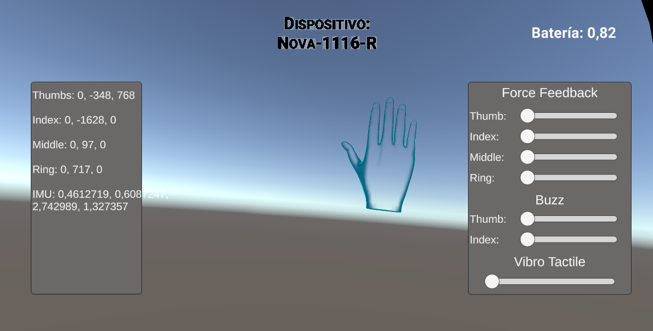
\includegraphics[width=0.9\textwidth]{hapticsmanager.PNG}
\caption{Escena de control de los guantes}
\end{figure}

\subsection{Fusionando Tecnologías}
Llegado a este punto, di un paso más allá en mi camino hacia el desarrollo de VR\cite{VR} con Unity, estableciendo la primera conexión del dispositivo Oculus Quest 2 y sus controladores Touch a una escena desarrollada por mí. Esta escena llamada por mí \textit{oculusTesting}, la utilicé para llevar a cabo algunas pruebas. Aquí trabajamos para ver que nos ofrecían y para que podemos usarlas. 
En este punto enfrentamos algunas complicaciones, ya que era necesario usar los plugins tanto de Oculus como de XR y cambiar algunos ajustes del software para que funcionase correctamente.

Tras las pruebas, gracias a las posibilidades de tracking a partir de la componente Transform\cite{Transform} de Unity pudimos obtener de una manera realista tanto datos de la posición en el espacio como de su rotación, lo cual nos fue útil para poder desarrollar dentro de nuestro proyecto. En este punto el movimiento de la cámara principal se encuentra enlazado al movimiento de nuestra visión desde las gafas, sincronizando así gafas de juego y la visión.

Aquí comencé a realizar una nueva escena, de nombre \textit{GloveAndOculus} donde buscaba adaptar la de diagnóstico y control háptico de los guantes a un uso conjunto con las gafas y controladores, pero cambiando el panel controlador por uno con datos del tracking de Oculus. Para conseguir esta adaptación fue fundamental el cambiar el tipo de interfaz de usuario dentro de la escena para que deje de ser estático en la pantalla (lo que provocaba fallos) y pase a verse desde las gafas Oculus (world space). Una vez conseguido esto, el siguiente paso que buscaremos será el de intentar representar las dos manos(con los guantes) y utilizar los controladores para trackear y establecer de manera real la posición y la rotación de las manos. Habrá que montar los Touch sobre los propios guantes.

Se consiguió el objetivo marcado en una escena llamada \textit{SeeingHands}, pero antes tuve que montar sobre el reverso de los guantes un soporte que contienen dentro del packaging del producto con el uso de unos tornillos que también venían. Fue necesario utilizar el tutorial que tienen en su página para poder montarlo correctamente. Esto es necesario por que al no tener los guantes posibilidad de tracking, montando unos controladores de VR\cite{VR} sobre ellos podemos cubrir esta opción. Tras este montaje, establecí las conexiones de los dispositivos a Unity, y desarrollé un pequeño script donde asignamos la componente\cite{Componentes} transform de los controladores a la del objeto de nuestros guantes(la representación digital de nuestras manos). Con esto y una opción que tiene el objeto de los guantes que permite especificar el tipo de controlador que se está usando, conseguimos que se vean las manos representadas de manera correcta en posición y rotación en el espacio. 

\section{Trabajo con Robótica}
En esta sección veremos el desarrollo y trabajo con el brazo robótico Kinova, lo dividiremos en dos instancias, una en la que trabajamos de manera simulada con una replicación virtual y otra, de manera real.
\subsection{Trabajo sobre Simulación}
Llegados a este punto lo que queríamos era llevar a cabo la replicación virtual de lo que sería el robot real. Para ello utilizamos un diseño de una pinza robótica hecha por nuestros compañeros dentro de esta escena. Las funciones que ejecturía el brazo realmente son la de desplazamiento en el espacio y la apertura/cierre de la pinza. A través de un script de nombre \textit{VirtualRobot} se implementaron los métodos get y set de la posición en las tres dimensiones del espacio y de la apertura de esta pinza para poder abrirla y cerrarla. En este apartado tuve complicaciones, que se solventaron profundizando en el estudio de la documentación de Unity centrándome en la parte de rotation y sus valores/tipos de datos de la componente Trnasform. Utilizo una variable de nombre \textit{Apertura} que unifica la rotación de la componente X de cada brazo de la pinza de manera que se muevan simultáneamente, simulando el movimiento real de abrir y cerrar la pinza. 
\begin{figure}[h]
\centering
\label{Cierre y apertura total de la pinza robótica}
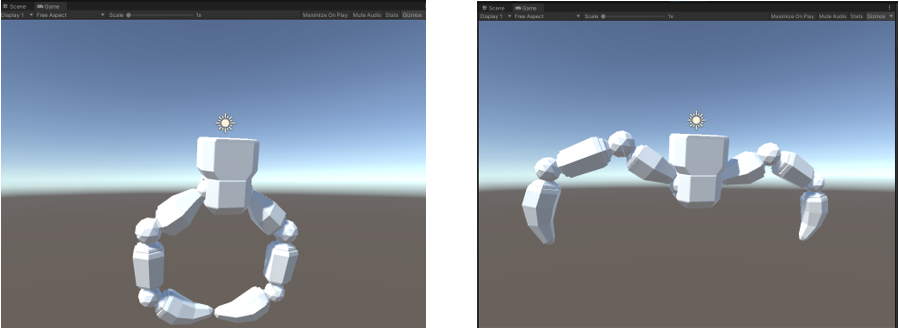
\includegraphics[width=0.9\textwidth]{img/pinza open close.PNG}
\caption{Cierre y apertura total de la pinza robótica}
\end{figure}
 Posteriormente la escena de replicación virtual de la pinza del robot fue mejorada implementándose dentro del script además de los getters y setters, dos métodos de movimiento. El primero de ellos en el espacio, dada una velocidad lineal y una posición objetivo, se mueve desde su origen hasta allí con esa velocidad. También se implementó el segundo, que controla el movimiento de apertura de la pinza, también dada una velocidad para la apertura y seleccionando una apertura objetivo. 
 
 El siguiente paso era hacer funcionar la pinza y desplazarla con nuestras manos, para ello creé una nueva escena en la que unimos la parte desarrollada para poder tener nuestras manos representadas en el espacio en tres dimensiones y con sus movimientos, junto con lo desarrollado para la pinza del robot. Para conseguirlo ha sido desarrollado el script \textit{Connector} el cual se encarga de hacer de puente de conexión entre guantes y la pinza. La lógica que se ha aplicado es que la pinza siga el desplazamiento de la mano gracias a la función de movimiento y la velocidad fijada, pero a una posición cercana para poder tener ambas cosas en vista. Además, ha sido implementada la idea de que al hacer con nuestros guantes el gesto de cerrar índice y pulgar, la pinza simule ese movimiento con la apertura que indiquemos con nuestro guante y a la velocidad de apertura marcada. Esto lo hemos podido conseguir gracias a recoger los datos de las flexiones de los dedos con nuestro script \textit{GettingData} que llevamos a cabo al principio.
 
 \subsection{Trabajo real}
Llegados a este punto, comenzamos con la integración del robot en el proyecto, primero realizamos una serie de pruebas desde otro proyecto en unity y después ya en el propio del TFG donde he creado una nueva escena de nombre \textit{ROSConnector} desde la cual con los scripts nos comunicaremos con nuestro robot. El funcionamiento de la escena es el siguiente:

En primer lugar, un objeto \textit{ROSInitializer} que contiene la componente del script de mismo nombre al que le daremos el dato de la IP del robot, en este caso 192.168.50.103 y el dato de número de puerto, para poder establecer la conexión. Hijos de este objeto, otros dos. Uno será un objeto para probar Kinova al que se le asocia un \textit{ROSInitializer} y el nombre de servicio. Y el otro el controlador Kinova que nos permite mandar instrucciones de desplazamiento tanto angular como linear al brazo y regular la apertura de la pinza. 

En cuanto a la conexión física del robot previa a Unity, utilizamos un router que se encuentra conectado a mi pc y a un switch que a su vez está conectado a la red. Para ello dentro de las opciones de configuración del adaptador de red, en el apartado TCP/IPv4 tenemos que seleccionar manualmente la subred que nos permita comunicarnos con el robot. Gracias a hacer ping y usar el comando \textit{ipconfig} podemos comprobar que todo esté correcto.

Para poder saber, entender y aprender como utilizar el robot entramos dentro de él gracias a establecer la conexión a través del SSH\cite{SSH} a la dirección IP del robot. Hubo que cambiar por medio de Nmtui la opción de asignación red del robot a automática y buscarla por su número de MAC en el escáner de redes. Desde aquí podemos acceder a información del robot y, utilizando el comando \textit{rostopic list} se nos muestra toda la lista de posibles comandos que podemos usar para interactuar con él. Esta lista se cribó para ver cuáles eran útiles para nuestro objetivo.

Finalmente, fuimos a por el último objetivo fusionando todo lo aprendido y desarrollado. La última escena contiene tanto la parte de VR y conexión al dispositivo Oculus y sus controllers, como la conexión a los guantes hápticos y como no, la conexión al robot. El objetivo de esta escena será, finalmente, controlar el robot con nuestro controller Oculus\cite{Quest2} montado sobre el guante, para así mover el brazo robótico en el espacio y cerrar y abrir la pinza solo con tener el guante puesto. 

Para alcanzar el objetivo de esta escena ha sido necesario, a nivel de software, el escribir un Script al que he llamado \textit{BotHandsLinking}. Este script es el manager que gestiona esta escena, ya que permite trabajar sobre el Kinova Position Controller que tenemos desarrollado anteriormente, al que le envía los datos del controller Oculus (referidos a la posición) para mover el brazo en el espacio. Se restringen los valores y se aplican offsets, de cara a una mejor experiencia de usuario. El controlador de posición es un script que publica en un topic los mensajes con las posiciones objetivo en los ejes X Y Z del robot.
Además se controla también la rotación de la mano.

Para finalizar el desarrollo del proyecto de fin de grado, ha sido añadido un script a esta última escena llamado \textit{GripManager} que se encarga de aplicar sobre una componente del robot que se ocupa de publicar los mensajes relacionados con la apertura o cierre de la pinza del robot, la lógica utilizada en las escenas previas. Esta lógica toma los valores recogidos por los guantes en los dedos y aplica el cierre o apertura deseado sobre la pinza del robot.


\capitulo{6}{Trabajos relacionados}

La teleoperación nació junto con la industria nuclear en los años 50 debido a la necesidad de manejar materiales altamente radioactivos , muy peligrosos para la salud simplemente con estar en su presencia. 
En los años setenta la teleoperación alcanzó su madurez con su aplicación en misiones espaciales, concretamente en los vehículos a control remoto Lunojod I y Lunojod II enviados a la Luna en 1970 y 1973 respectivamente.

En las últimas décadas, los avances en teleoperación han ido muy ligados a la evolución de la robótica y la informática. Gracias a estos avances, muchos sistemas de teleoperación actuales consisten en robots que tienen una gran autonomía y solo precisan ser teleoperados para determinadas acciones que, debido a las limitaciones de la robótica, no pueden realizar por si solos. También se ha progresado en las interfaces hombre-máquina buscando una mayor sensación de control de la máquina y de telepresencia.

Los robots tele-operados pueden encontrarse en la industria nuclear (mantenimiento de reactores), química (manejo a distancia de sustancias peligrosas o tóxicas), militar (detección, manipulación y desmantelamiento de cargas explosivas), desminado humanitario, espacial (exploraciones realizadas en la luna y en marte, también en transbordadores espaciales), minera (excavaciones, manejo de cargas explosivas en minas y túneles), en el sector de seguridad, mantenimiento y rescate (inspección de sistemas de alcantarillado y tuberías, reconocimiento de zonas de desastres), telecirugía , entre muchas otras áreas.

\newpage
Algunos ejemplos de proyectos realizados son:
\begin{itemize}
    \item \textbf{Proyecto H2020 Sarafun}\cite{Sarafun} : se investigaron las habilidades sensoriales y cognitivas de vanguardia para un robot, así como habilidades de razonamiento necesarias para planificar y ejecutar una tarea de ensamblaje.
    \item \textbf{Proyecto JAK\&Teleoperación}\cite{JAK} : se planteó un sistema que permite al usuario describir y controlar el robot desde una simulación basada en realidad virtual
    \item La compañía \textbf{SET}\cite{Set}  está desarrollando un sistema para operar robots remotamente que permitiría operar estos elementos aunque estén en el espacio
\end{itemize}

\capitulo{7}{Conclusiones y Líneas de trabajo futuras}
Para finalizar tanto esta memoria como el proyecto destinado a ser mi trabajo de fin de grado de la carrera de Ingeniería Informática vamos a llevar a cabo una pequeña conclusión y también veremos algunas de las posibles líneas de trabajo y de investigación futuras.

\section{Conclusiones}
Llegados a este punto podemos hablar de una conclusión de los objetivos de manera correcta. Satisfaciendo tanto lo esperado como lo marcado por los requisitos para el software del proyecto. Por la naturaleza del proyecto, el cual es eminentemente de investigación podríamos haber topado con problemas y errores que no nos permitieran alcanzar todo lo marcado. En cambio podemos afirmar que se encuentra desarrollado un software a través del motor\cite{MotorGrafico} gráfico Unity\cite{Unity}, que nos permite conectar un sistema de dispositivos de realidad virtual\cite{VR} compuesto por unas gafas, Oculus Quest 2 con sus controladores, y unos guantes hápticos Nova con un robot para ser teleoperado mediante nuestra mano y a través de gestos.

Se alcanzó a conseguir todos los objetivos marcados como principales, algunos de los secundarios, los marcados de carácter técnico y de los que personalmente me siento muy orgulloso que son los objetivos marcados como personales.

Todo este proceso de desarrollo del proyecto ha sido concluido con éxito, pero por el camino he enfrentado momentos más complicados, principalmente al principio, ya que no tenía la experiencia suficiente de trabajo con las herramientas con las que ha sido desarrollado el proyecto ni con las metodologías aplicadas.
Considero con un carácter fundamental el hecho de haber cursado la mayor parte de un curso de desarrollo con Unity antes de empezar el proyecto, ya que sin esta formación me hubiera sido imposible desarrollar.

Las 300 horas marcadas para la resolución del mismo me han resultado justas, ya que en caso de no haber podido completar a tiempo alguno de los sprints, podría haberme visto sin tiempo para concluir el desarrollo de la manera esperada. Además estas 300 horas han sido en un 95\% de su totalidad dedicadas al desarrollo, el resto a documentar y elaborar tanto esta memoria como el anexo. Por lo tanto me he visto necesitando de muchas horas más por mi cuenta para poder acabar estos documentos.

No tenía ninguna experiencia previa trabajando ni con Unity, ni con C\#, ni con robots, ni con tecnologías de realidad virtual. Pero puedo asegurar que esta experiencia de trabajo ha sido positiva, enriquecedora y satisfactoria para mi. También destaco el uso de \LaTeX para documentar, ya que es una herramienta que permite generar documentación de una manera sencilla pero estéticamente perfecta.

Desde este punto debo dar las gracias tanto a la Universidad de Burgos como a ITCL, ya que sin ambos dos no hubiera podido adentrarme en un proyecto de esta magnitud, con un elevado coste presupuestario y un desarrollo tan especial. Dar las gracias también a mi tutor empresarial Alejandro Langarica Aparicio ya que ha sido un gran mentor y ejemplo a la hora de trabajar y resolver problemas, y a Carlos Cambra Baseca por ser mi tutor universitario de este TFG.

Además quisiera aprovechar este espacio para dar las gracias al resto de profesores que me han formado para poder alcanzar este momento y esta entrega. 
Indudablemente debo agradecer a mis padres, a mi hermano Pablo, a Julia, a los vatos, a mis amigos cercanos y a todo aquel que me dio fuerza para llevar a cabo este trabajo, por ser una fuente tanto de inspiración como de energía para mi.

\newpage

\section{Líneas de Trabajo Futuras}
Algunas de las posibilidades de trabajo de cara al futuro que se contemplan desde este punto del proyecto son:

\begin{itemize}
    \item Recibir respuesta háptica al operador en relación a variaciones en
el estado del robot o su entorno.
    \item Desarrollar un sistema de visión estereoscópico ajustable y sincronizado al movimiento de cabeza del operador
    \item Desarrollar una interfaz para superponer sobre la imagen virtual que tiene el teleoperador, en vista de dotar de más funcionalidades.
    \item Proyectar un sistema inalámbrico de comunicación basado en la nube para el control remoto.
\end{itemize}


\bibliographystyle{plain}
\bibliography{bibliografia}

\end{document}
